\documentclass[11pt]{beamer}
\usetheme{Warsaw}
\usepackage[utf8]{inputenc}
\usepackage[english]{babel}
\usepackage{amsmath}
\usepackage{mathabx}
\usepackage{mathtools}
\usepackage{qtree}
\usepackage{amsfonts}
\usepackage{amssymb}
\author{Joe Duffin}
\title{A Theorem Proving Assistant}
\setbeamercovered{transparent} 
\setbeamertemplate{navigation symbols}{} 
\titlegraphic{
\includegraphics[width=0.9cm]{logo}} 
\institute{School of Computer Science \\University College Dublin} 
\date{20th March 2017} 
\subject{Final Year Project Presentation} 
%\setbeamertemplate{footline}[page number]

\begin{document}

\setlength{\abovedisplayskip}{0pt}
\setlength{\belowdisplayskip}{0pt}
\setlength{\abovedisplayshortskip}{0pt}
\setlength{\belowdisplayshortskip}{0pt}

\begin{frame}
\titlepage
\end{frame}

%\begin{frame}
%\tableofcontents
%\end{frame}

%%%%%%%%%%%%%%%%%%%%%%%%%%%%%%%%%%%%%%%%%%%%%%%%%%%%%%%%%%%%%%%%%%%%
\begin{frame}{Overview}
\begin{itemize}
\setlength\itemsep{2em}
\item What is Theorem Proving
\item What I Built
\item How does it work
\end{itemize}
\end{frame}

%%%%%%%%%%%%%%%%%%%%%%%%%%%%%%%%%%%%%%%%%%%%%%%%%%%%%%%%%%%%%%%%%%%%
\begin{frame}{What is a Theorem?}
A Theorem is a proposition which is not necessarily self-evident but can be proved with a chain of reasoning.\\
\vspace{1cm}
\begin{Theorem}[$\vee zero$]
$P \vee true \equiv true$
\end{Theorem}
\end{frame}

%%%%%%%%%%%%%%%%%%%%%%%%%%%%%%%%%%%%%%%%%%%%%%%%%%%%%%%%%%%%%%%%%%%%
\begin{frame}{What is Theorem Proving?}

\begin{columns}[c] 

\column{.45\textwidth} % Left column and width
\begin{block}{Proof of $\vee zero$}
\begin{align*}
&P \vee true \\
\equiv&\ \ \{(X:\coloneqq P).(0)\} \\
&P \vee ( P \equiv P ) \\
\equiv&\ \ \{(X,Y,Z\coloneqq P,P,P ).(1)\} \\
&P \vee P \equiv P \vee P \\
\equiv&\ \ \{(X \coloneqq P).(2)\} \\
&P \equiv P \\
\equiv&\ \ \{(X \coloneqq P).(0)\} \\
& true
\end{align*}
\end{block}

\column{.5\textwidth} % Right column and width
\begin{block}{Theorems}

$(0) [X \equiv X \equiv true ]$\\
$(1) [X \vee (Y\vee Z) \equiv (X\vee Y) \vee Z]$\\
$(2) [X \vee X \equiv X]$

\end{block}

\end{columns}

\end{frame}

%%%%%%%%%%%%%%%%%%%%%%%%%%%%%%%%%%%%%%%%%%%%%%%%%%%%%%%%%%%%%%%%%%%%
\begin{frame}{What I Built}
\begin{figure}
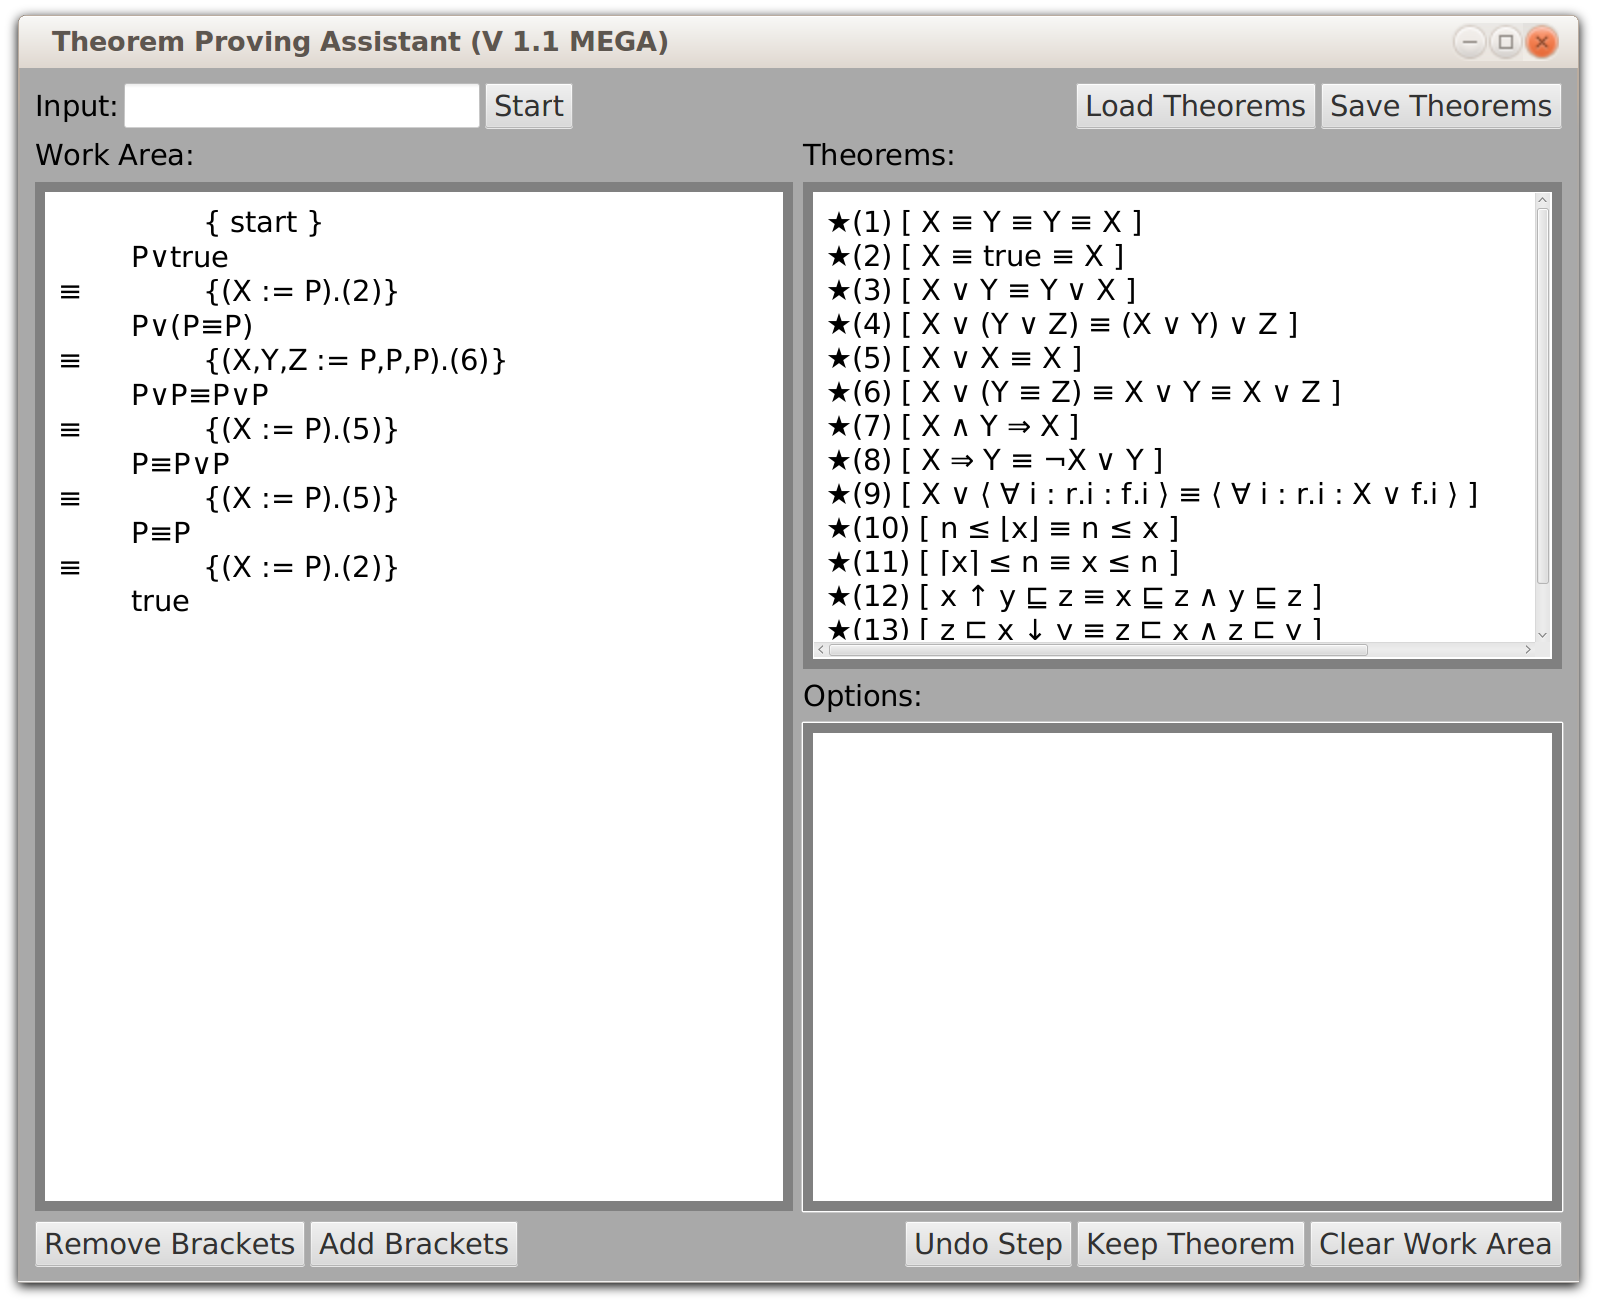
\includegraphics[width=0.8\linewidth]{../TheReport/screenshot}
\end{figure}
\end{frame}

%%%%%%%%%%%%%%%%%%%%%%%%%%%%%%%%%%%%%%%%%%%%%%%%%%%%%%%%%%%%%%%%%%%%
\begin{frame}{How it Works - Expression Representation}
\begin{columns}[c]

\column{.45\textwidth} % Left column and width
\begin{block}{String Representation ($\vee zero$)}
$P \vee true \equiv true$
\end{block}
\begin{block}{Tree Representation ($\vee zero$)}
\Tree [.$\equiv$  [ P true !{\qbalance} ].$\vee$ true ]\\
\end{block}

\column{.5\textwidth} % Right column and width
\begin{itemize}
\item Syntax trees are used to represent expressions.
\end{itemize}
\end{columns}
\end{frame}

%%%%%%%%%%%%%%%%%%%%%%%%%%%%%%%%%%%%%%%%%%%%%%%%%%%%%%%%%%%%%%%%%%%%
\begin{frame}{How it Works - Pattern Matching}

\end{frame}

%%%%%%%%%%%%%%%%%%%%%%%%%%%%%%%%%%%%%%%%%%%%%%%%%%%%%%%%%%%%%%%%%%%%
\begin{frame}
\Huge{\centerline{Questions...}}
\end{frame}
\end{document}